%------------------------------------------------------------------------%
\chapter{BJT}
%------------------------------------------------------------------------%


\centering
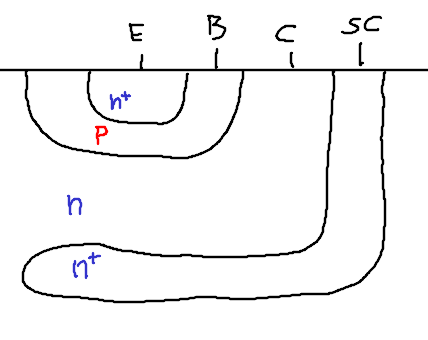
\includegraphics[width=0.35\textwidth]{bjt1.png}\\
\raggedright

This device is created with 2 pn junctions with a back to back connection creating a npn or a pnp device. This device can be horizontal or vertical (we will study this second approach beacuse is the most important).\\
The n structure is the collector the $n^+$ is the sub-collector region connected to the surface with a reach-throught implantation. The current flows in the vertical direction so the most significant part is the one under the collector area.\\
The main idea is to forward bias the EB-j and reverse bias the BC-j. Foward bias in EB-j so there will be a flow of electrons form E to B holes to B-E but if the base region is narrow we have that electrons don't recombine in the p region but travel throught it reaching the collector.\\
We have a large flow of electrons throght a reverse biased junction (BC) beacuse the supply comes from the EB-j and not from GR processes. In the collector we have high resistivity due to low doping concentrations so we have to put the sub-collector to make a contact.\\
\vspace{5mm}
This device has a significant flow of both electrons and holes so it's a bipolar device (intrinsic flow of holes from base to emitter).\\
We can minimize the base current by reducing the width of the base and olso making the emitter more doped wrt the base.\\
\vspace{5mm}
If the BC-j was direct biased we will have an additional component to the base current that is something we want to avoid.\\

\section{Doping concentrations}

\centering
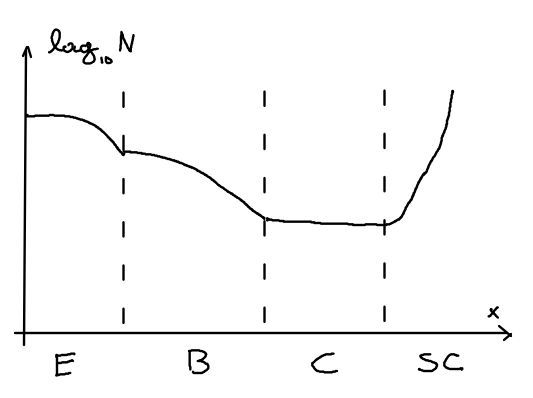
\includegraphics[width=0.35\textwidth]{bjt2.png}\\
\raggedright

Let's analyse the doping concentrations; in emitter region we have high doing concentration $N_d^E\simeq 10^{20}$ that decrease until $10^{18}$, the base from $N_a^B=10^{18}$ to $10^{17}$ and then the collector and the subcollector as in figure. The non constant doping concentration is relevant in the operation of the device.\\
 
\section{Collector current}
We can focus our analysis on the quasi-neutral p region that is the bottom-neck for conduction of the system.

\centering
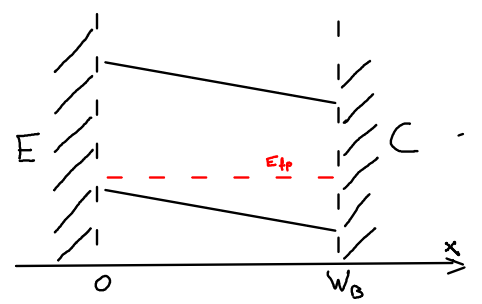
\includegraphics[width=0.35\textwidth]{bjt3.png}\\
\raggedright

We call $W_b$ the quasi neutral region of the base. In this region the band banding is set by holes concentration. Doping concentration is not constant so we have a band banding like in figure so a F due to non constant doping concentrations. This condition can be reached olso with high level of injection.\\
Considering hole concentration $p=n_ie^{\frac{E_i-E_{fp}}{kT}}$ we get $E_i=E_{fp}+kT\ln(p/n_i)$. We want this parameter beacuse it's releted to the potential and so to the electric field
\begin{equation}
F=-\frac{d\phi}{dx}=\frac{1}{q}\frac{dE_{i}}{dx}=\frac{1}{q}\frac{dE_{fp}}{dx}+\frac{kT}{q}\frac{1}{p}\frac{dp}{dx}
\end{equation}
both high injection and non constant doping concentration events are taken into account by the term $\frac{dp}{dx}$, the term $\frac{dE_{fp}}{dx}$ take into account of resistive drops.\\
\vspace{5mm}
The base current density is $J_B=p\mu_p \frac{dE_{fp}}{dx}$ so we get that $\frac{dE_{fp}}{dx}=J_p/(p\mu_p)$ and so putting this equation into the electric field equation we get 
\begin{equation}
\frac{1}{q}\frac{J_p}{p\mu_p}+\frac{kT}{q}\frac{1}{p}\frac{dp}{dx}
\end{equation}
using some reasonable values for all the parameter we get that $\Delta V_t$ is of a few fractions of mV when the total voltage applied is in the order of 0.6-0.7V. This contribution is negligible we consider the $E_{fp}$ almost constant so 
\begin{equation}
F=\frac{kT}{q}\frac{1}{p}\frac{dp}{dx}
\end{equation}

\vspace{5mm}
We can recover the drift-diffusion expression for the current and using F we get
\begin{equation}
J_n=qn\mu_n \frac{kT}{q}\frac{1}{p}\frac{dp}{dx}+qD_n \frac{dn}{dx}
\end{equation}
We are in a quasi neutral region so $p(x)=N_a(x)+n(x)$ we can get 2 cases.\\
\vspace{3mm}
\tab {\bf Low injection}\\
$n<<N_a$ so the expression for the current is 
\begin{equation}
J_n=qn\mu_n \frac{kT}{q}\frac{1}{N_a}\frac{dN_a}{dx}+qD_n \frac{dn}{dx}
\end{equation}
where $\frac{kT}{q}\frac{1}{N_a}\frac{dN_a}{dx}$ is the built in electric field due to non constant doping concentration.\\
\vspace{3mm}
\tab {\bf High injection}\\
$n>>N_a$ so we get 
\begin{equation}
J_n=qn\mu_n \frac{kT}{q}\frac{1}{n}\frac{dn}{dx}+qD_n \frac{dn}{dx}=2qD_n\frac{dn}{dx}
\end{equation}
it's like a pure diffusion process with the double of the intesity; this is called the Webster effect.\\


%------------------------------------------------------------------------%
\subsection{Prototype BJT current}

\centering
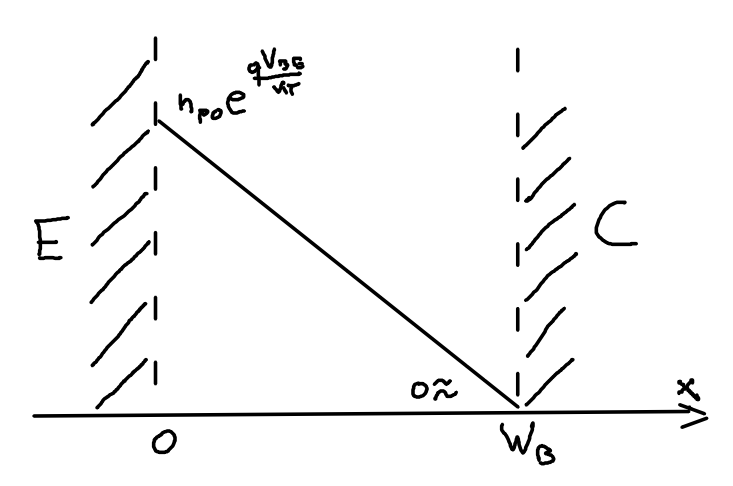
\includegraphics[width=0.35\textwidth]{bjt4.png}\\
\raggedright

It's a super-ideal case where we have constant doping concentrations and low level of injection.\\
So we have that $J_n=qD_n \frac{dn}{dx}$; we can say as "boundary conditions" that $n(0)=\frac{n_i^2}{N_a}e^{qV_{BE}/kT}$ and that $n(W_b)=\frac{n_i^2}{N_a}e^{qV_{BC}/kT}$ but beacuse $V_{BC}<0$ we can say that $n(W_b)\simeq 0$.\\
Now we can integrate the two members and since $J_n$ is a constant becuse there isn't recombination we get
\begin{equation}
J_n=qD_n\frac{n(W_b)-n(0)}{W_b}
\end{equation}
that is legit beacuse $\frac{dn}{dx}$ it's a linear profile we are considering a narrow base diod.\\
\begin{equation}
J_n=-\frac{qD_nn_i^2}{N_aW_b}e^{qV_{BE}/kT}
\end{equation}
We can now multiply for the area of the emitter $A_E$ and add a minus sign beacuse we want current positive if flows into the collector arriving at
\begin{equation}
I_c=A_E\frac{qn_i^2}{\frac{N_aW_b}{D_n}}e^{qV_{BE}/kT}=A_E\frac{qn_i^2}{G_B}e^{qV_{BE}/kT}
\end{equation}
where $G_B=\frac{N_aW_b}{D_n}$ it's the Gummel number of the base.\\
This current it's dependent only on base parameters.

%------------------------------------------------------------------------%
\subsection{"Ideal" BJT}

We consider now the possibility of non constant doping concentration or high injection regime so we recover the expression $J_n=qn\mu_n \frac{kT}{q}\frac{1}{p}\frac{dp}{dx}+qD_n \frac{dn}{dx}$ that we can write as
\begin{equation}
J_n=\frac{qD_n}{p}\left(n \frac{dp}{dx}+p \frac{dn}{dx}\right)= \frac{qD_n}{p}\frac{d(pn)}{dx}
\end{equation}
As before we integrate keeping $J_n$ as a constant we know that $pn(W_d)\simeq 0$ so we reach the current density as 
\begin{equation}
J_n=-\frac{qn_i^2}{\int^{W_b}_0 \frac{p}{D_n}dx}e^{qV_{BE}/kT}
\end{equation}
If we multiply for the emitter area and change sign we get the collector current as 
\begin{equation}
I_c=A_E\frac{qn_i^2 e^{qV_{BE}/kT}}{\int^{W_b}_0 \frac{p}{D_n}dx}=A_E\frac{qn_i^2 e^{qV_{BE}/kT}}{G_B}
\end{equation}
where $G_B=\int^{W_b}_0 \frac{p}{D_n}dx$ is the new Gummel number for the base that in case of constant doping and low level of injection becomes the first one.\\

%------------------------------------------------------------------------%
\subsection{Real BJT}

The most general case we can include the non-constant bandgap in the base. We can have a non constant bandgap due to 2 causes.\\
The first cause of bandgap narrowing is due to doping conectrations that are higher than $\simeq 10^{18}$; high doping means donor closer to each other interaction between energy levels that becomes a band of energy and some of this level can overlap the $E_c$ narrowing the band-gap. The emitter side we will have a narrower gap than the collector side.\\

\centering
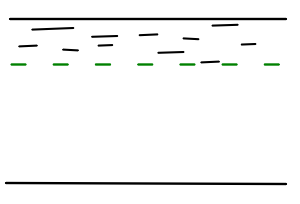
\includegraphics[width=0.2\textwidth]{bjt5.png}\\
\raggedright

Second cause is a technological method to gradually change from Si to GeSi to narrow the bandgap ($E_{gap}^{Ge}<E_{gap}^{Si}$).

\centering
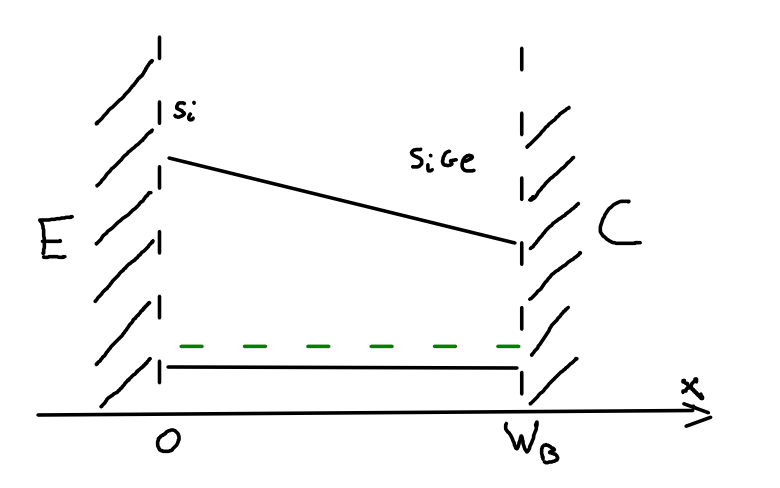
\includegraphics[width=0.4\textwidth]{bjt6.png}\\
\raggedright

In all the calculation we have an important role of the bangap only in $pn=n_i^2e^{(E_{fn}-E_{fp})/kT}$ in this the intrinsic carrier concentration becomes
\begin{equation}
n_{i,e}^2=N_vN_ce^{-E_{gap}/kT}e^{\Delta E_{gap}/kT}=n_i^2e^{\Delta E_{gap}/kT}
\end{equation}
where $n_{i,e}$ is the effective intrinsic carrier density. 
So $J_n=n\mu_n \frac{dE_{fn}}{dx}$ where from the previous equation and the generalized law of mass action we get 
\begin{equation}
E_{fn}=E_{fp}+kT\ln(\frac{pn}{n_{i,e}})
\end{equation}
considering $E_{fp}$ constant as usual we get that the current density is 
\begin{equation}
J_n=qD_n \frac{n_{i,e}^2}{p}\frac{d(pn/n_{i,e}^2)}{dx}
\end{equation}
as the previous case now we integrate this expression 
\begin{equation}
J_n=-\frac{qe^{qV_{BE}/kT}}{\int^{W_b}_0 \frac{p}{D_nn_{i,e}^2}}dx
\end{equation}
Multiplying the result for the emitter area and changing the sign we get the collector current as 
\begin{equation}
I_c=A_E \frac{qn_i^2 e^{qV_{BE}/kT}}{\int^{W_{b}}_0\frac{n_i^2p}{n_{i,e}^2D_n}dx}=A_E \frac{qn_i^2 e^{qV_{BE}/kT}}{G_B}
\end{equation}


%------------------------------------------------------------------------%
\section{Base current}
%------------------------------------------------------------------------%

Base current created by holes that moves from base to emitter region. In our analysis we will consider emitter region beacuse it's the bottom neck for conduction in this process.

\centering
{\bf Figure 107mancante}\\
\raggedright
%------------------------------------------------------------------------%
\subsection{Shallow emitter}
We can neglect recombination of holes and so $J_p=const$.\\
We will refer to the most general case of high level of injection, non constant doping concentration and gap narrowing.\\
From the consideration made for the collector current we get $J_p=-qD_p \frac{n_{i,e}^2}{n}\frac{d(pn)}{dx}$ and as boundary condition we know that $p(0)=p_{n0}e^{qV_{BE}/kT}$ and at the contact $p(-W_e)=p_{n0}$.\\
Making one step of integration (and neglecting 1) we get 
\begin{equation}
J_p=-e^{qV_{BE}/kT}\frac{1}{\int_{-W_e}^0 n/(qD_nn_{i,e}^2) dx}
\end{equation}
From this we get the base current
\begin{equation}
I_B= A_E e^{qV_{BE}/kT}\frac{n_i^2}{\int_{-W_e}^{0}\frac{n n_i^2}{n_{i,e}^2D_n} dx}=A_Ee^{qV_{BE}/kT}\frac{n_i^2}{G_E}
\end{equation}
where $G_E$ is the Gummel number of the emitter. All base current parameter are function of the emitter.\\
We will never reach high injection condition beacuse the emitter is highly doped so we can write
\begin{equation}
G_E= \frac{N_d^En_i^2}{n_{i,e}^2D_n}W_B 
\end{equation}

%------------------------------------------------------------------------%
\subsection{Deep emitter}
In the case of constant doping an low level of injection from pn-j results neglecting -1 we get
\begin{equation}
J_p=-{\frac{qD_pn_i^2}{N_d^EL_p\tanh(W_e/L_p)}e^{\frac{qV_{BE}}{kT}}}
\end{equation}
and so the base current as
\begin{equation}
I_B=A_E \frac{qn_i^2}{\frac{N_d^E L_p \tanh(W_e/L_p)}{D_p}}e^{qV_{BE}/kT}=A_E \frac{qn_i^2}{G_E}
\end{equation}
where $G_E=\frac{N_d^EL_p \tanh(W_e/L_p)}{D_p}$ it's the new Gummel number of the emitter. \\
Now we can calculate the beta of the transistor as
\begin{equation}
\beta=\frac{I_C}{I_B}=\frac{G_E}{G_B}
\end{equation}

%------------------------------------------------------------------------%
\section{$\beta$ dependance on $I_C$}
%------------------------------------------------------------------------%

\centering
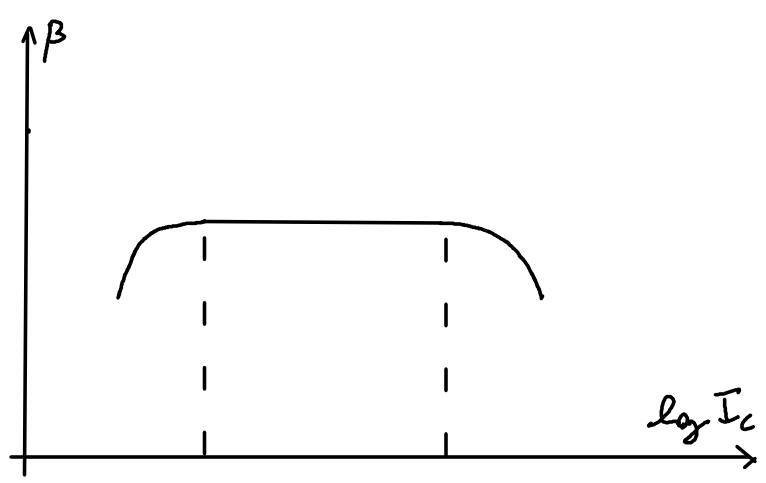
\includegraphics[width=0.25\textwidth]{bjt7.png}\\
\raggedright

$\beta$ changes with different $I_C$ values at high current and low current we can see a drop of this parameter.

\centering
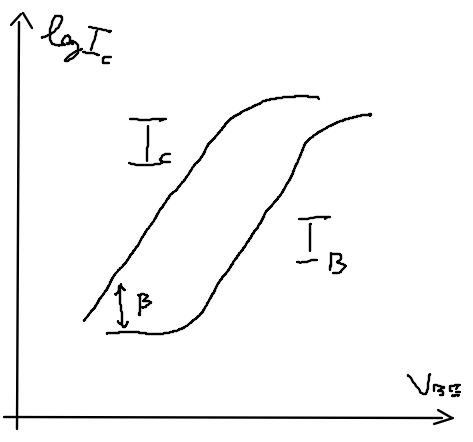
\includegraphics[width=0.35\textwidth]{bjt8.png}\\
\raggedright

Plotting the Gummel plot for the BJT that at low current the base current drops slowly reducing $\beta$ while at high current both $I_C$ and $I_B$ deviate from ideal characteristic.\\
\vspace{3mm}
At low current we have GR processes of the forward biased EB junction in the depletion layer.
\vspace{3mm}
In high current we have high injection effects and resistive drops. The high injection effects affect only $I_C$ for the low doping of the base region. This is called modulation of the base conductivity.\\

%------------------------------------------------------------------------%
\section{Kirk effect}
Consider now the BC junction under the condition of constant doping concentration. We get the results of a pn junction.\\
The total charge in the quasi neutral region is 0 but in the depletion zone we have some localized charge and so an electric field as shown in the figures below.\\
The area of the triangle of F profile has to be constant and proportional at $\Delta \phi=\phi_{bi}+V_{CB}$.\\

\centering
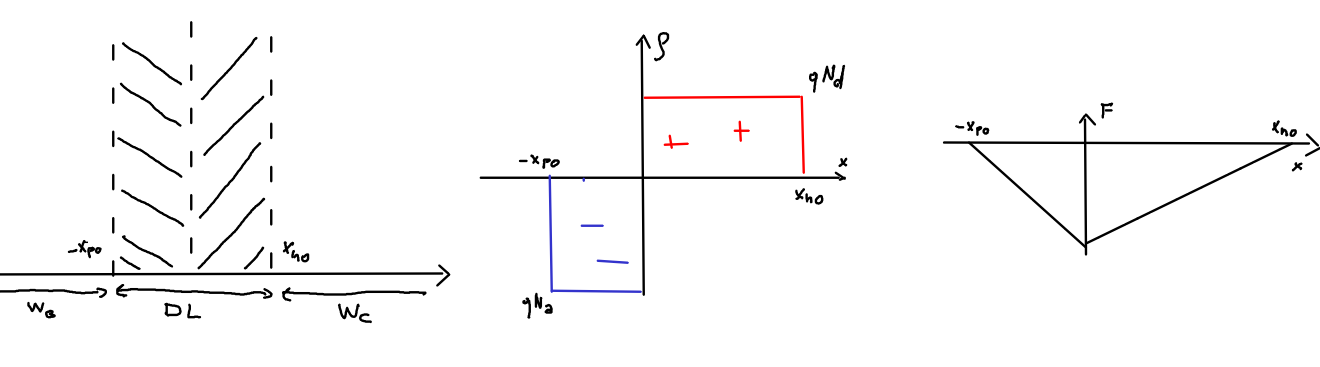
\includegraphics[width=0.8\textwidth]{bjt9.png}\\
\raggedright

All this results are based on the depletion approximation but in this case we have the EB-j that forces a large (and indipendent on $V_{BC}$) flow of electrons.\\
Electrons move by drift (we are in a reverse bias junction) and we can suppose they move at the saturation velocity so $J_n=qnv_{sat}$ form which we can write that $n=J_n/qv_{sat}$; if $J_n$ increase olso n increase until it's comparabple with $N_d^C$ and in this case the depletion approximation is no more valid.\\
The slope of the second part of F becomes from $\frac{qN_d^C}{\varepsilon_{si}}$ to $\frac{q(N_d^C-n)}{\varepsilon_{si}}$ we are reducing the slope but the area has to remain constant so we decrease also the elcetric field.\\

\centering
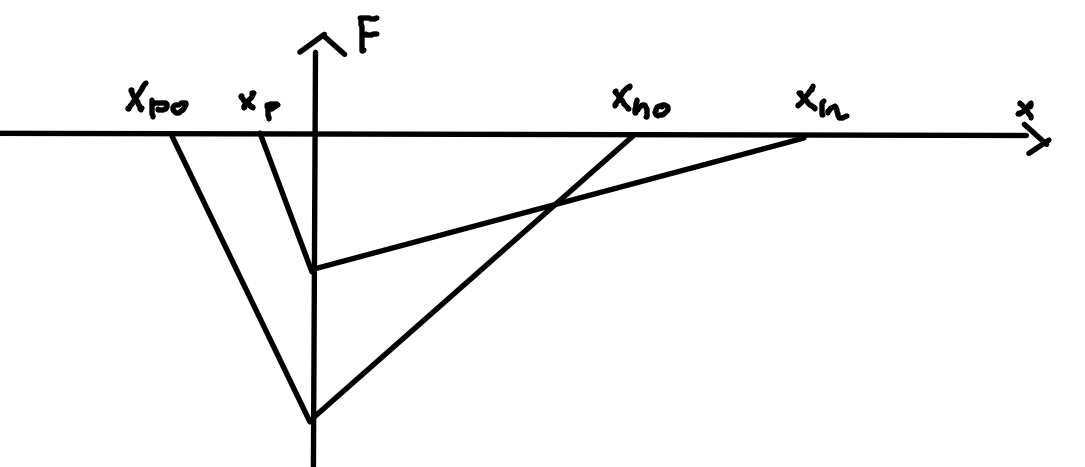
\includegraphics[width=0.35\textwidth]{bjt10.png}\\
\raggedright

We have so doing a wider $W_B$ the Gummel number of the base increase and so the collector current decreases.\\
This is called Kirk effect and does not affect the base current.\\
\vspace{5mm}

In the beginning case we can say that $x_{p0}N_a^B=x_{n0}N_d^C$ and from this that 
\begin{equation}
W_{d0}=\sqrt{\frac{2\varepsilon_{Si}}{q}\Delta\phi(\frac{1}{N_a^B}+\frac{1}{N_d^C})} \ \ \ \ \ \ \ \ \ \Delta \phi=W_{d0}^2 \frac{q}{2\varepsilon_{Si}} N_a^B//N_d^C
\end{equation}
but when we have non negligible n we get $x_{p0}(N_a^B+n)=x_{n0}(N_d^C-n)$ and from that 
\begin{equation}
\Delta \phi=W_{d0}^2 \frac{q}{2\varepsilon_{Si}}\frac{(N_a^B+n)(N_d^C-n)}{N_a^b+N_d^C}
\end{equation}
combining this 4 equations we get the real distances 
\begin{equation}
x_n=x_{n0}\sqrt{\frac{1+n/N_a^B}{1-n/N_d^C}}\simeq x_{n0}/\sqrt{1-n/N_d^C}
\end{equation}
\begin{equation}
x_p=x_{p0}\sqrt{\frac{1-n/N_d^C}{1+n/N_a^B}}\simeq x_{p0}\sqrt{1-n/N_d^C}
\end{equation}

We can increase more the quasi-neutral base region. If we keep increasing n we arrive that the depletion layer in the collector reaches the subcollector (where it stops for high doping of this region) like in the graph.\\
Increasing more the depletion layer moves to the C-SC junction making $W_B$ a lot wider and so having a drop of $\beta$ and of the frequency responce.\\
The onset of this event can be found at current $J_n=qnv_{sat}=qN_d^C v_{sat}$

\centering
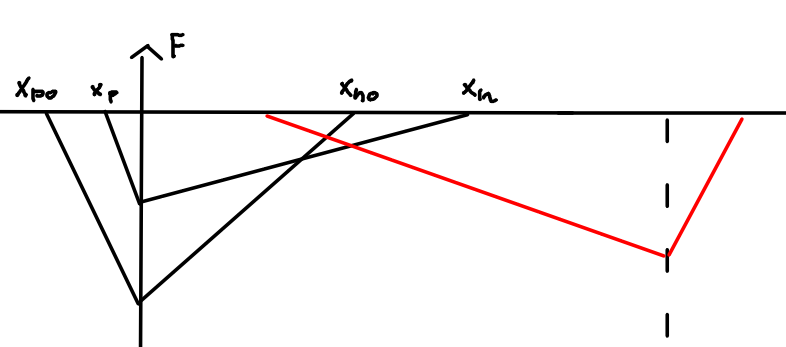
\includegraphics[width=0.35\textwidth]{bjt11.png}\\
\raggedright


%------------------------------------------------------------------------%
\section{Early effect}
%------------------------------------------------------------------------%

\centering
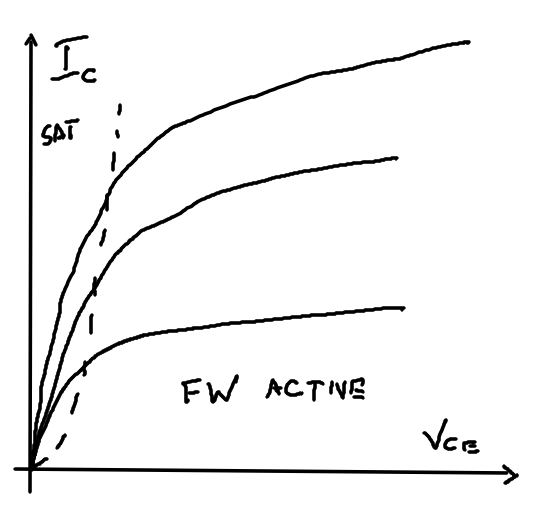
\includegraphics[width=0.15\textwidth]{bjt12.png}\\
\raggedright

Now we want to investigate the dependances of $I_C$ on $V_{CE}$ so we focus on the qn base region and we keep $V_{BC}$ not big and negative.\\
If $V_{CE}=0$ than $V_{BE}=V_{BC}$ so constant electron concentration and no diffusion current (accounting for base current it isn't really zero but slightly negative).
Increasing $V_{CE}$ we reduce forward bias on BC decrease electron concentration at the BC depletion region so the current increase and we enter in the forward active mode leaving the saturation regime.

\centering
{\bf Figure 111}\\
\raggedright

In the forward active mode we have a slight increase of the current the physical reason for this comes from the qn region of the base; increasing $V_{CE}$ at constant $V_{BE}$ we are moving the width of the depletion layer in the base increasing F profile and so the diffusion current. This is the Early effect of the BJT.\\

\centering
{\bf Figure 112mancante}\\
\raggedright

We follow the rect until the interception with the x axes where we find $-V_A$ the Early voltage.\\
The slope of the rect is $\frac{\partial I_C}{\partial V_{CE}}$ given a certain $\hat{I_C},\hat{V_{CE}}$ we can say that $\frac{\partial I_C}{\partial V_{CE}}=\hat{I_C}/(V_A+\hat{V_{CE}})$ and so neglecting $\hat{V_{CE}}$ that is small
\begin{equation}
V_A=\frac{\hat{I_C}}{\frac{\partial I_C}{\partial V_{CE}}}
\end{equation}
we can say that $\frac{\partial I_C}{\partial V_{CE}}|_{V_{BE}}=\frac{\partial I_C}{\partial V_{CB}}$ and so
\begin{equation}
\frac{\partial I_C}{\partial V_{CB}}=-\frac{-\hat{I}}{W_B}\frac{\partial W_B }{\partial V_{CB}}
\end{equation}  
where
\begin{equation}
\frac{\partial W_B }{\partial V_{CB}}=-\frac{\partial x_{p0}}{\partial V_{CB}}\frac{qN_a^B}{qN_a^B}=-\frac{C_{dep}^{BC}}{qN_a^B}
\end{equation}
where the minus sign is for coherence with the prototype transistor current.
Finally we get
\begin{equation}
V_A=\frac{qN_a^BW_B}{C_{dep}^{BC}}=\frac{Q_p}{C_{dep}^{BC}}
\end{equation}
$Q_p$ total base charge of holes.\\
To increase $V_A$ it's better to act on $C_{dep}^{BC}$.
The lower limit for the width of the base is to avoid the punch-throught regime that is when the entire base is depleted.\\

%------------------------------------------------------------------------%
\section{Small signal model}
%------------------------------------------------------------------------%

%------------------------------------------------------------------------%
\subsection{Trasconductance}
Variation of $I_C$ with a small variation of $V_{BE}$ at constant $V_{CE}$ 
\begin{equation}
g_m=\frac{\partial I_C}{\partial V_{BE}}|_{V_{CE}}=\frac{I_C}{kT/q}
\end{equation}

%------------------------------------------------------------------------%
\subsection{Output resistance}
Variation of $I_C$ with variation of $V_{CE}$ at constant $V_{BE}$ to the minus one 
\begin{equation}
r_0=\left(\frac{\partial I_C}{\partial V_{CE}}|_{V_{BE}}\right)^{-1}=\frac{V_A}{I_C}
\end{equation}

%------------------------------------------------------------------------%
\subsection{Base resistance}
How $I_B$ change with small change of $V_{BE}$ at constant $V_{CE}$
\begin{equation}
r_{\pi}=\left(\frac{\partial I_B}{\partial V_{BE}}|_{V_{CE}}\right)^{-1}=\frac{\beta}{g_m}
\end{equation}
Note that $\frac{\partial I_B}{\partial V_{CE}}|_{V_{BE}}=0$.\\

%------------------------------------------------------------------------%
\subsection{Capacitive effects}
We have 2 capacitance $C_\pi=C_{dep}^{BE}+C_{diff}$ ,where $C_{diff}$ comes from the modulation of free carrier charge inside the device, and $C_\mu=C_{diff}^{BC}$.\\
We only miss the value of $C_{diff}$. We can analyse first $Q_{diff}=Q_B+Q_E+Q_{BC}+Q_{BE}$ where $Q_{BC}$ is for the Kirk effect $Q_B,Q_E$ come from the quasi neutral region of the base and collector.\\
\vspace{5mm}
$\rightarrow$ $Q_B=I_Ct_b$ where $t_b$ is the transit time of minority carriers. From pn junction's results we get that $t_b=W_b^2/2D_n$.\\
\vspace{2mm}
$\rightarrow$ Considering a deep emitter we get $Q_E=I_B\tau_p=I_C \frac{\tau_p}{\beta}=I_Ct_e$ where $t_e$ time related to emitter region (not transit time of course). \\
\vspace{2mm}
$\rightarrow$ $Q_{BC}$ free charge stored in BC depletion region that is
\begin{equation}
Q_{BC}=q \frac{J_n}{qv_{sat}}W_d^{BC}A_E=I_C \frac{W_d^{BC}}{v_{sat}}=I_C t_{BC}
\end{equation}
$\rightarrow$ For $Q_{BE}$ we can't use the previous results beacuse we have diffusion process but we say it's $Q_{BE}=I_Ct_{BE}$. It's a negligible contribution.\\
\vspace{5mm}
So $Q_{diff}=I_C(t_b+t_e+t_{bc}+t_{be})=I_C \tau$ and finally
\begin{equation}
C_{diff}=\frac{\partial Q_{diff}}{\partial V_{BE}}=g_m\tau
\end{equation}

\centering
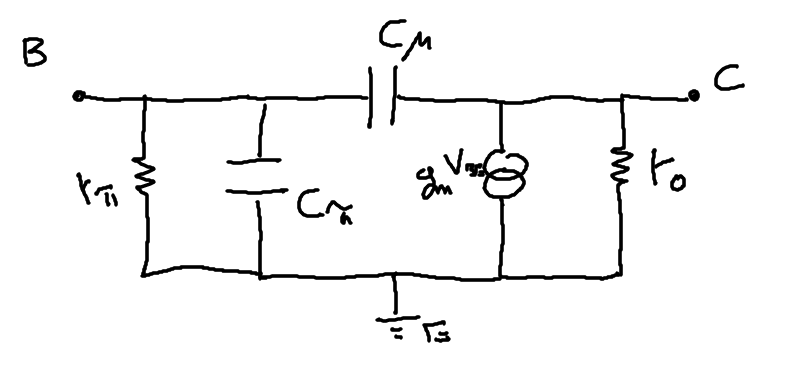
\includegraphics[width=0.35\textwidth]{bjt13.png}\\
\raggedright


%------------------------------------------------------------------------%
\section{Frequency responce}
%------------------------------------------------------------------------%

The cut off frequancy is
\begin{equation}
f_t=\frac{g_m}{2\pi(C_\pi+C_\mu)}
\end{equation}
having $g_m$ means dependance on the collector current so we can make the invers of the equation and plot a graph to better undestand the frequancy responce
\begin{equation}
\frac{1}{f_t}=\frac{2\pi(C_{dep}^{BE}+C_{dep}^{BC})}{I_C}\frac{kT}{q}+2\pi\tau
\end{equation}

\centering
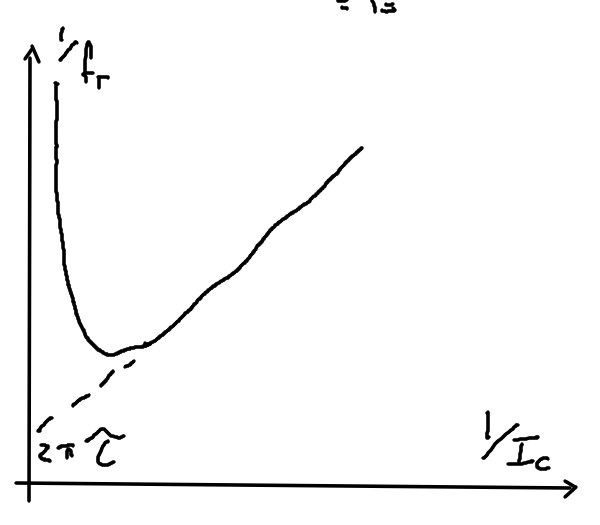
\includegraphics[width=0.35\textwidth]{bjt14.png}\\
\raggedright

At too high current we enter in high current regime triggering base widening and Kirk effect that decrease our frequency responce.\\



%------------------------------------------------------------------------%
\section{Considerations}
%------------------------------------------------------------------------%

If we want to increase $I_C$ we have to increase $N_d^C$ to avoid Kirk and work at higher frequency but to not worst the Early effect we have to increase olso $N_d^B$ but at this point olso $N_d^E$ to not decrease $\beta$.\\
\vspace{5mm}
We want low variability of $\beta$ so a deep emitter with the consequents strange process technology as in figure.\\

\centering
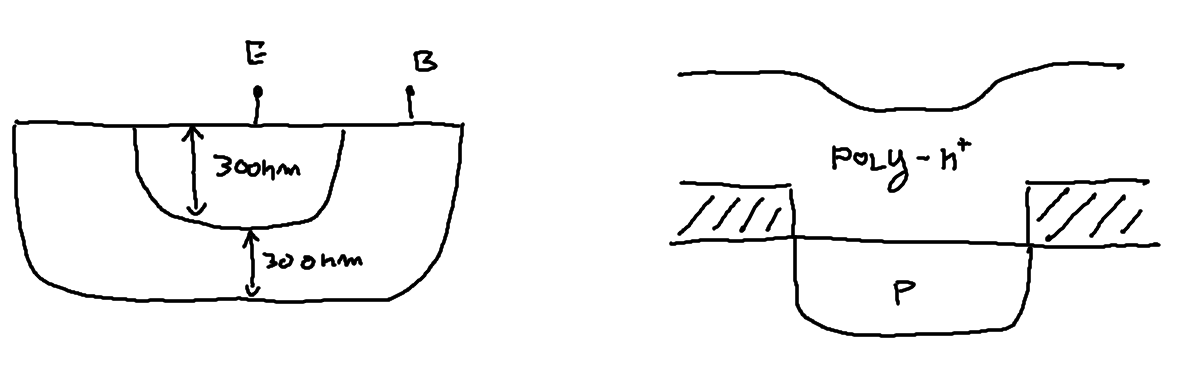
\includegraphics[width=0.45\textwidth]{bjtfinal.png}\\
\raggedright

We aren't able due to process tollerance to make an emitter deep 300nm and a base only 10nm they have to be of the same dimensions if we don't use particular pocesses like in the second figure. With this method we can have a very deep emitter made of $n^+-$polysilicon deposited at last and a shallow base that is doped as first process.\\
With this technology we can arrive at $f_t\simeq 100GHz$.\\

\vspace{5mm}
With C-mos technology we have to trade the maximum gain with high frequency regimes but in bjt technology no; this is why bjt's are still used for analog circuits.\\
In a simple amplifier with a BJT the maximum gain is $G_{max}=g_m r_0=V_a/(\frac{kT}{q})\simeq 1000$ that is indipendent on the working current. In a MOS amplifier we have $G_{max}=V_a/\left(\frac{V_{gs}-V_t}{m}\right)\simeq100$ that is lower but we can olso write that as 
\begin{equation}
G_{max}=\sqrt{\mu_nC_{ox}WL2/m}\frac{F_P}{\sqrt{I_{ds}^{sat}}}
\end{equation}
that shows us the trade off between maximum gain and frequency responce.


\vspace{130mm}
\raggedleft
{\it ...that's all for today see you tomorrow!}
